 \documentclass[a4paper, twocolumn]{article}
%\documentclass[a4paper]{article}
\makeatletter
\def\@seccntformat#1{%
  \expandafter\ifx\csname c@#1\endcsname\c@section
  \thesection $\mid$
  \else
  \csname the#1\endcsname\quad
  \fi}
\makeatother
\usepackage{tikz}
\usetikzlibrary{positioning,arrows,automata}
\usepackage{abstract}
\usepackage{fullpage}
\usepackage[utf8]{inputenc}
\usepackage[english]{babel}
\usepackage{lipsum}
\usepackage{amsmath}
\usepackage{amsfonts}
\usepackage{pgf, tikz}
\usepackage{pgfplots}
\usepackage{float}
\usepackage{listings}
\usepackage{xcolor}
\usepackage{tabularx}
\usepackage{hyperref}
\usepackage[all]{xy}
\usetikzlibrary{fit,arrows.meta}
\usetikzlibrary{automata, positioning}


% FOR THE CODE IN SECTION 5 
\definecolor{codegreen}{rgb}{0,0.6,0}
\definecolor{codegray}{rgb}{0.5,0.5,0.5}
\definecolor{codepurple}{rgb}{0.58,0,0.82}
\definecolor{backcolour}{rgb}{0.95,0.95,0.92}

\lstdefinestyle{mystyle}{
    backgroundcolor=\color{backcolour},
    commentstyle=\color{codegreen},
    keywordstyle=\color{magenta},
    numberstyle=\tiny\color{codegray},
    stringstyle=\color{codepurple},
    basicstyle=\ttfamily\scriptsize,
    breakatwhitespace=false,
    breaklines=true,
    captionpos=b,
    keepspaces=true,
    numbers=left,
    numbersep=5pt,
    showspaces=false,
    showstringspaces=false,
    showtabs=false,
    tabsize=2
}

\usepackage{titlesec}

\setcounter{secnumdepth}{4}
\titleformat{\paragraph}
{\normalfont\normalsize\bfseries}{\theparagraph}{1em}{}
\titlespacing*{\paragraph}
{0pt}{3.25ex plus 1ex minus .2ex}{1.5ex plus .2ex}

\lstset{style=mystyle}

\title{\textbf{Security analysis of Corona Tracing Applications}}
\date{\textbf{-- BSP6 --}\\Summary\\ \today}
\author{
    Maria ZHEKOVA\\
    \small University of Luxembourg\\
    \small\texttt{maria.zhekova.001@student.uni.lu}
	\and
    Marjan SKROBOT\\
    \small University of Luxembourg\\
	\small\texttt{marjan.skrobot@uni.lu}
	%\and
	%Yan KIM\\
	%\small University of Luxembourg\\
	%\small\texttt{yan.kim@uni.lu}
}

\begin{document}
\maketitle

% ---------- 1| INTRODUCTION ---------- 
\section{Introduction}
Nowadays COVID-19 pandemic has become one of the most common subjects for discussion. More countries adopt COVID-19 tracing systems to track contacts of infected users. With the corona tracing applications development and the way users are being tracked arise security and privacy risks. Thus the reason of our project. 
% ---------- 2| CONTEXT ---------- 
\section{Context}
The project consist in designing and implementation of a system representing a corona tracing application which at the end should be analysed and verified. For the modeling and verification we use a model checker called Uppaal \cite{uppaal}. The description of a model in Uppaal consist of three parts: global and local declarations, automata templates and a system definition.

% ---------- 3| Requirements analysis --------- 
\section{Requirements analysis} 
For this project we had few requirements.\\
Before all, we needed to have deeper understanding on the different system architectures of corona tracing applications and their protocols. In order to provide an analysis and verification, we needed to be familiar with topics such as model checking, system verification and formal languages. Before starting to design in a model checker we needed to represent the system in a formal language such as LTL. The model checking tool Uppaal should have also been understood for a successful deliverance of such system verification.

% ---------- 4| Design ---------- 
\section{Strategy}
In this section we will briefly define some of the important knowledge for the production of the project.
\subsection{Corona tracing app design}
There are three distinct architectures of COVID-19 tracing apps; centralized, decentralized and hybrid. The actors of such systems are the user, server and authority.\\
Each user has a set of specific ID’s or only one ID, used to send to the close-by users as an encounter message. 
When an user is labelled as COVID- 19-positive from a diagnosis facility, the server may receive all the encounters of the user from the last few days, keeping in mind that first the user should be verified of being COVID-19-positive via the authority.\\
The architectures have different properties and ways to transmit the encounters.\\
In the centralized architecture there is the risk of data leakage since the user gives upon registration his/hers name, telephone number, postcode etc, it is easier to create a social graph than in the other designs. If the encounter messages in the centralized architecture leak, the identity of user and his/hers contacts is revealed, but the adversary could be only the server.\\ 
The decentralized architecture is seen as less vulnerable to tracking attacks such as social graphs. If the encounter messages in the decentralized system leak, only the identity of the user leaks, but the adversary could be anyone. All users can access the public server to download the seeds and since the uploaded seeds are being uploaded together, a malicious entity can keep collecting them and link the identifiers. Only an infected user uploads the seeds, and therefore someone making traffic analysis can easily detect who is this infected person.\\
The hybrid architecture adopts advanced enhancement methods such as secret sharing and uses Diffie Hellman. In general, a user’s secret is shared between the user and the server. Since part of the infection risk analysis is computed at the server using privacy preserving secret sharing, if one party is compromised, the entire secret or risk analysis result will not be revealed. In addition devices keep full control over the secret identifiers which makes them less vulnerable to breaches at the server\\

\noindent For this project, we chose to design a decentralized system with the Decentralized Privacy-Preserving Proximity Tracing (DP-3T) protocol \cite{dp3t-white}\cite{dp3t}.\\

\noindent More details could be found in the main report in our GitHub repository \cite{github}.
\subsection{Methods}
A very important aspect when designing a system is the verification of that system. There is defined a specific process for model checking with three phases as can be seen on Figure \ref{fig:modelCheck}.\\
The first one is the modelling phase, where we model the system and a property for verification using the language of the model checker.\\
The second phase is the running phase, where we actually verify the property.\\
The final phase is the analysis phase, where if the phase two resulted in success we can define a new property. If, however phase two resulted in failure, we need to analyse the model and find the mistake.

% ---------- 5| Production ---------- 
\section{Production}
In this section we will briefly define a system verification as shown in the main report and in the demonstration.\\
We do not have designed the Server, nor the authority, but the model of the user does include a state that can be used if a Server or Authority are included. Therefore our system consist only in users exchanging ephermal ids \texttt{EphID} as their encounter messages and adversaries. The system was verified with the help of two queries.
\subsection{User}
At the beginning the user chooses location and a COVID-19 status (positive, negative, possible positive).The set of \texttt{EphID}s is predefined and the user must choose at the start of the day his/hers \texttt{EphID}with checking the possible maximum number of \texttt{EphID} per day. Then starts the broadcasting. If possible, the user can change to another \texttt{EphID} or go to the next day by repeating the process from the beginning.

\subsection{Adversary}
In our system we have designed two adversaries. One adversary can capture the broadcasted encounters from everywhere and transmit them to every location possible, without considering the location of the adversary. The other adversary can capture encounters only from the same location as the adversary itself, but when changing location, the adversary can broadcast the already captured encounters from another location to the new one.

\subsection{Query}
In order to verify the designed system we used two queries for two similar verifications.\\
The first one verifies if every time that and user receives an \texttt{EphID}, it is received from another user and not its own and if it is a bidirectional communication.\\
The second query is similar to the one above, but in addition to the previous one, it also looks up at the location. Thus it verifies again the same property as above but also if the received \texttt{EphID} is from an user in the same location.

% ---------- 6| Assessment ---------- 
\section{Assessment and Conclusion}
There was only one element of the requirements which was not completely satisfied. This element was the LTL representation of the model. However, the absent representation in a formal language did not affect our design and verification of the system in Uppaal.\\ Following the method for system verification we could successfully verify the system for the given properties with the help of the two queries.\\
Therefore we consider the project as successfully completed.

\newpage
\begin{thebibliography}{9}

\bibitem{uppaal}
Department of Information Technology at Uppsala University, Sweden \& the Department of Computer Science at Aalborg University in Denmark, "About Uppaal", [Online]. Available: \url{https://uppaal.org} [Accessed 18th of April 2021]

\bibitem{github}
M.Zhekova, M.Skrobot, Y.Kim, "Security analysis of Corona Tracing Applications", [Online]. Available:  \url{https://github.com/mzhekova97/BSP6-zhekova-maria} [Accessed 21st of June 2021]

\bibitem{dp3t-white}
"DP-3T White paper",[Online]. Available: \url{https://github.com/DP-3T/documents/blob/master/DP3T\%20White\%20Paper.pdf} [Accessed 1st of June 2021]

\bibitem{dp3t}
"DP3T - Decentralized Privacy-Preserving Proximity Tracing",[Online]. Available: \url{https://github.com/DP-3T/documents} [Accessed 1st of June 2021]

\end{thebibliography}
\newpage
% ---------- 7| APPENDIX---------- 
\section{Appendix} \label{appendix}
In this section can be found images related to the sections above.

\begin{figure}[h]
    \centering
    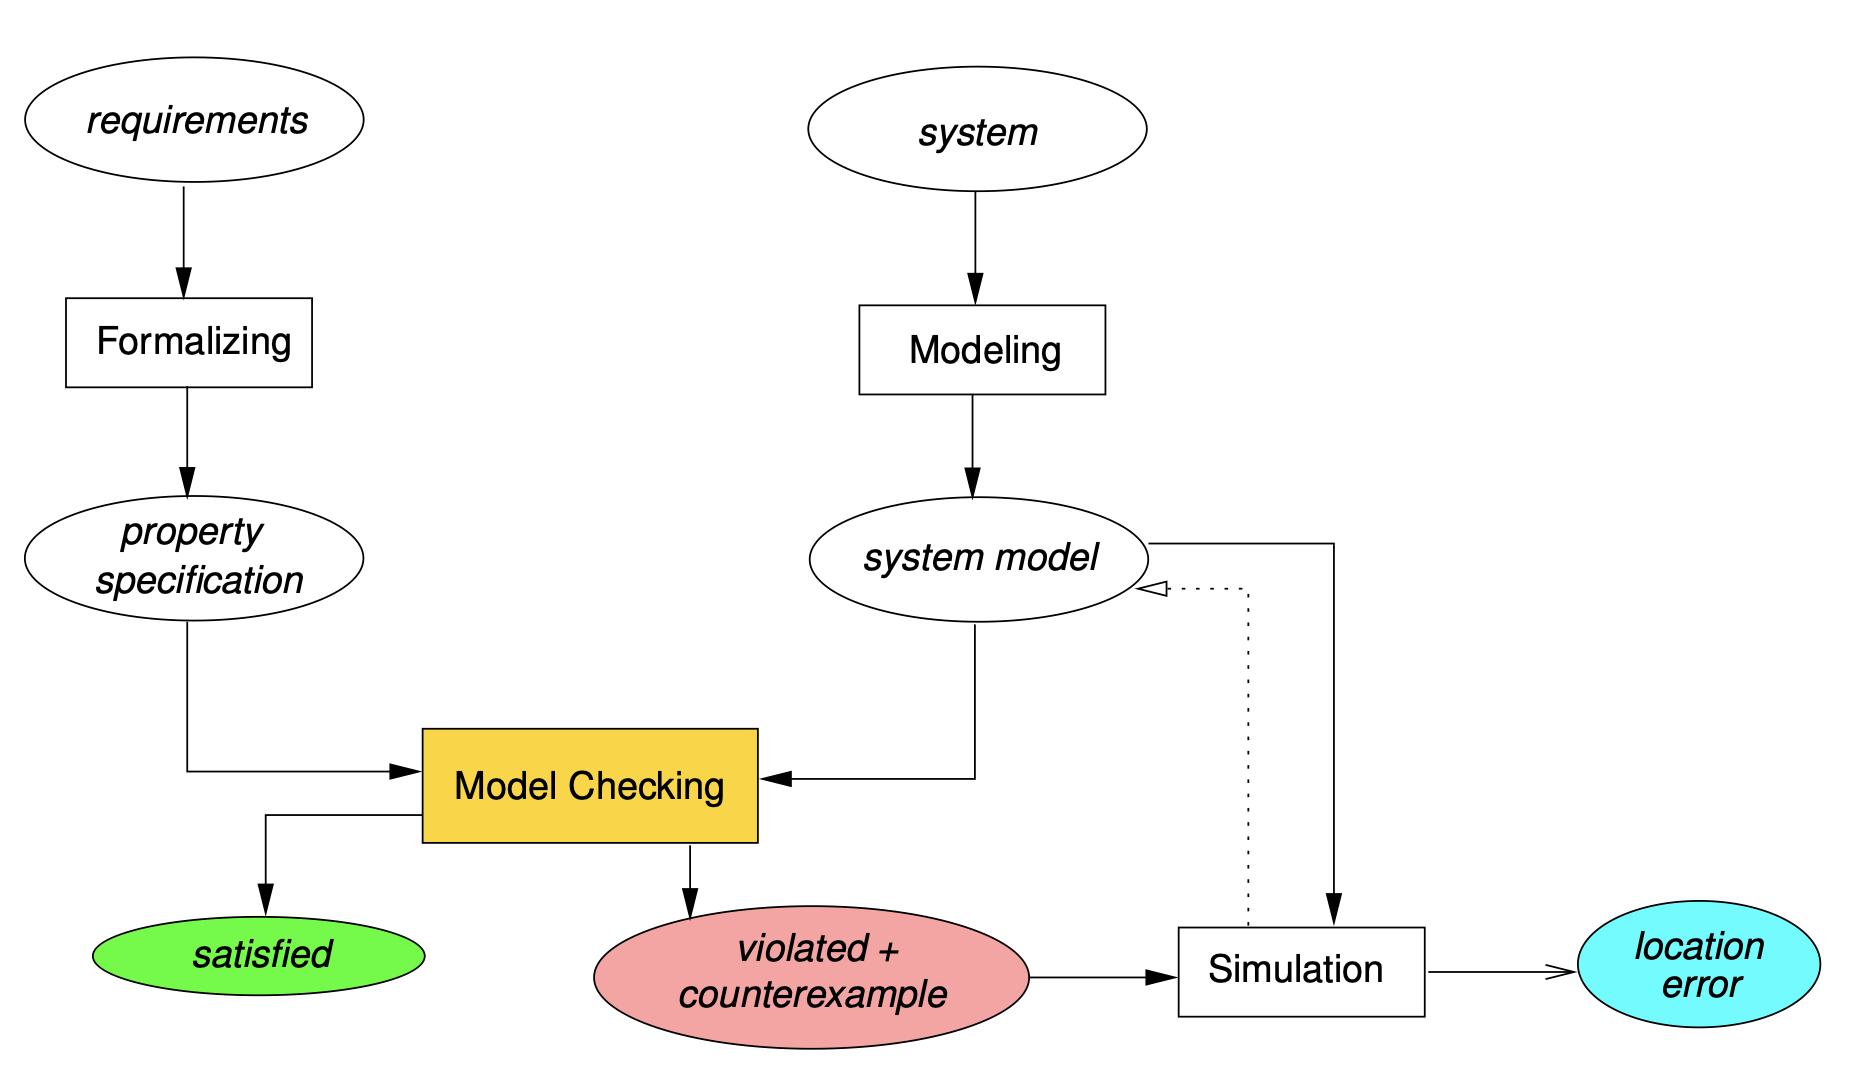
\includegraphics[scale=0.3]{images/modelCheck.png}
    \caption{Model Checking}
    \label{fig:modelCheck} 
\end{figure}
%\vspace{2em}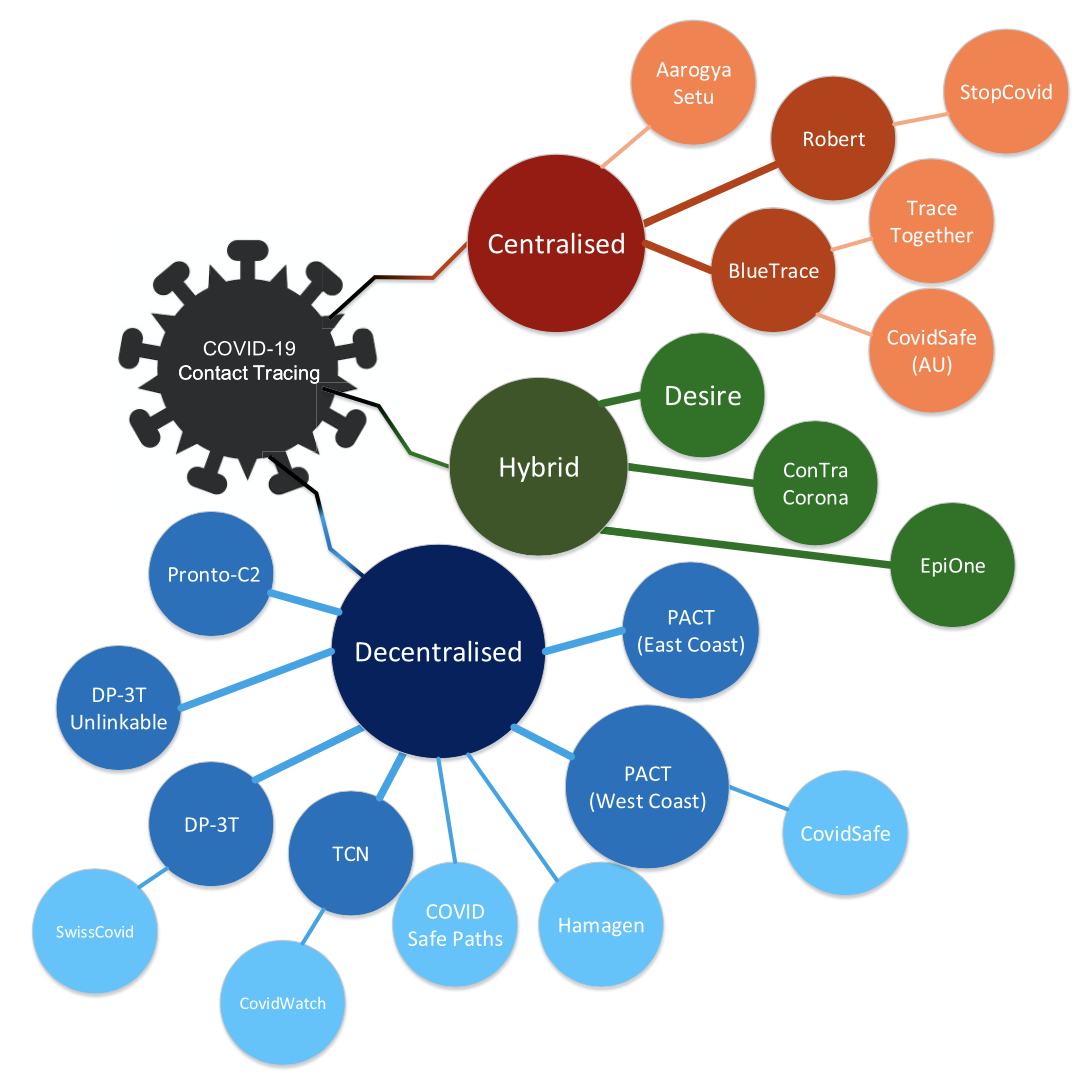
\includegraphics[scale=0.425]{images/protocolsApps.png}

\end{document}